\chapter{Modelos de iluminaci\'on para tejidos}
% Los materiales PBR \textit{MeshStandardMaterial} y \textit{MeshPhysicalMaterial} de ThreeJs funcionan muy bien para gran parte de
% materiales, como pl\'asticos o metales. Sin embargo carecen de par\'ametros que permitan representar fen\'onmenos como la
% dispersi\'on hacia delante y hacia detr\'as (\textit{forward/backward scattering}) o la absorci\'on y reflexi\'on interna (\textit{suburface scattering}) caracter\'isticos
% de gran cantidad de tejidos debido a la reflexi\'on de la luz con las fibras que lo componen.
Los tejidos se componen de fibras entrelazadas con cierta separaci\'on entre s\'i, por lo que la met\'afora de la
rejilla compuesta por microespejos que se utiliza en la teor\'ia de microfacetas no es la mejor aproximaci\'on para tratar
de representar este material de forma realista. Los materiales PBR \textit{MeshStandardMaterial} y \textit{MeshPhysicalMaterial} de
ThreeJs, basados en microfacetas, funcionan muy bien para gran parte de materiales, como pl\'asticos o metales, sin embargo no consiguen
una representaci\'on realista de tejidos, que suelen presentar un l\'obulo especular m\'as atenuado.\\

% La estructura de fibras puede provocar los efectos de absorci\'on y reflexi\'on interna (\textit{subsurface scattering}) y, dependiendo
% de la direcci\'on de la luz, los efectos de dispesi\'on hacia delante o hacia detr\'as (\textit{forward} y \textit{backward scattering}).
% Cuando la luz viene en direcci\'on opuesta al punto de vista y golpea las fibras que salen del tejido provoca el efecto de
% \textit{foward scattering}, mientras que cuando la luz viene en la misma direcci\'on que el punto de vista, el fen\'omeno
% de \textit{backward scattering}. El terciopelo es un caso de tejido en el que se acent\'ua este efecto y el primer trabajo en describirlo, el modelo de BRDF de Ashikmin
% \autocite{ashikhmin}, es tambi\'en conocido como \textit{velvet BRDF} o \textit{velvet distribution}.\\
La estructura de fibras puede provocar los efectos de absorci\'on y reflexi\'on interna (\textit{subsurface scattering}) y, dependiendo
de la direcci\'on de la luz, o los efectos de dispersi\'on hacia delante (\textit{forward scattering}) o hacia detr\'as (\textit{backward scattering}).
El efecto de \textit{forward scattering} se produce cuando la luz viene en direcci\'on opuesta al punto de vista y golpea las fibras que salen del tejido,
mientras que el \textit{backward scattering} se produce en la misma situaci\'on pero con la direcci\'on de la luz proviniendo del punto de vista. 
El terciopelo es un caso de tejido en el que se acent\'ua este efecto y el primer trabajo en describirlo, el modelo de BRDF de Ashikmin \autocite{ashikhmin}, es tambi\'en conocido como \textit{velvet BRDF} o
\textit{velvet distribution}.\\


Este trabajo implementa sobre ThreeJs el modelo de \textit{Cloth} de Filament \autocite{filament}. La librer\'ia de Google
presenta un BRDF especial para tejidos que, inspirado en los trabajos de Ashikmin \autocite{ashikhmin} y m\'as
tarde Estevez y Kulla \autocite{sheenbrdf} para el t\'ermino de distribuci\'on de las normales, y el de Neubelt \autocite{theorder}
para el factor de geometr\'ia, permite una representaci\'on realista en entornos interactivos de los efectos mencionados.

% al carecer de par\'ametros que permitan representar los fen\'onmenos de dispersi\'on hacia delante y hacia detr\'as (\textit{forward/backward scattering})
% o la absorci\'on y reflexi\'on interna (\textit{suburface scattering}), efectos caracter\'isticos de una amplia variedad de
% tejidos.\\

% Dependiendo de la direcci\'on de la luz con respecto al punto de vista, las fibras que componen los tejidos pueden provocar los
% efectos de \textit{forward scattering} cuando la luz viene de la direcci\'on opuesta al punto de vista y  \textit{backward scattering},
% cuando la luz viene desde la misma direcci\'on que el punto de vista. 

% Adem\'as la separaci\'on de las fibras puede 

% Adem\'as las ligeras separaciones


% los fen\'omenos de retrodispersi\'on o
% la reflexi\'on interna, compuestos de una gran cantidad de hilos que absorben y dispersan la luz.
% Es por ello que Filament presenta un nuevo BRDF basado en los trabajos de y que utiliza un par\'ametro de \textit{sheen} para
% que ofrece un control sobre el brillo especular para simular los fen\'omenos de reflexi\'on hacia delante y hacia detr\'as
% caracter\'istico de tejidos como el terciopelo. Adem\'as algunos materiales absorben parcialmente la luz y la emiten de nuevo,
% aport\'ando un color caracter\'istico determinado por las fibras del tejido, \'este fen\'omeno se representa con el par\'ametro
% \textit{subsurface} de Filament, que utiliza la aproximaci\'on conocida como \textit{wrapped diffuse lighting} \autocite{gpugems}\\


\section{Integraci\'on de una nueva clase de material en ThreeJs}
ThreeJs ofrece la posibilidad de crear materiales a trav\'es de su API, sin embargo, para este trabajo se ha decidido
crear un \textit{fork} de la librer\'ia para soportar posibles nuevos materiales y funcionalidades que se requieran
espec\'ificamente de Author.\\

En este cap\'itulo se explica la implementaci\'on de una nueva clase de material que se integra en la librer\'ia de materiales
de ThreeJs. Siguiendo la nomenclatura de la librer\'ia (\textit{MeshBasicMaterial}, \textit{MeshStandardMaterial}, etc.), el
nuevo material se llamar\'a \textit{MeshClothMaterial}.


% ThreeJs proporciona una API para extender de forma sencilla su librer\'ia de materiales, sin embargo, para proporcionar al nuevo
% material de la misma interfaz que los materiales nativos de ThreeJs, as\'i como seguir extendiendo la librer\'ia y ser flexible
% a futuros cambios, se ha optado por crear un \textit{fork} de la librer\'ia e introducir los cambios necesarios para crear
% este nuevo material.\\

% Siguiendo la nomenclatura de ThreeJs: \textit{MeshBasicMaterial}, \textit{MeshStandardMaterial}, etc., el nuevo material se
% llama \textit{MeshClothMaterial}.\\

\begin{figure}[H]
  \centering
    \frame{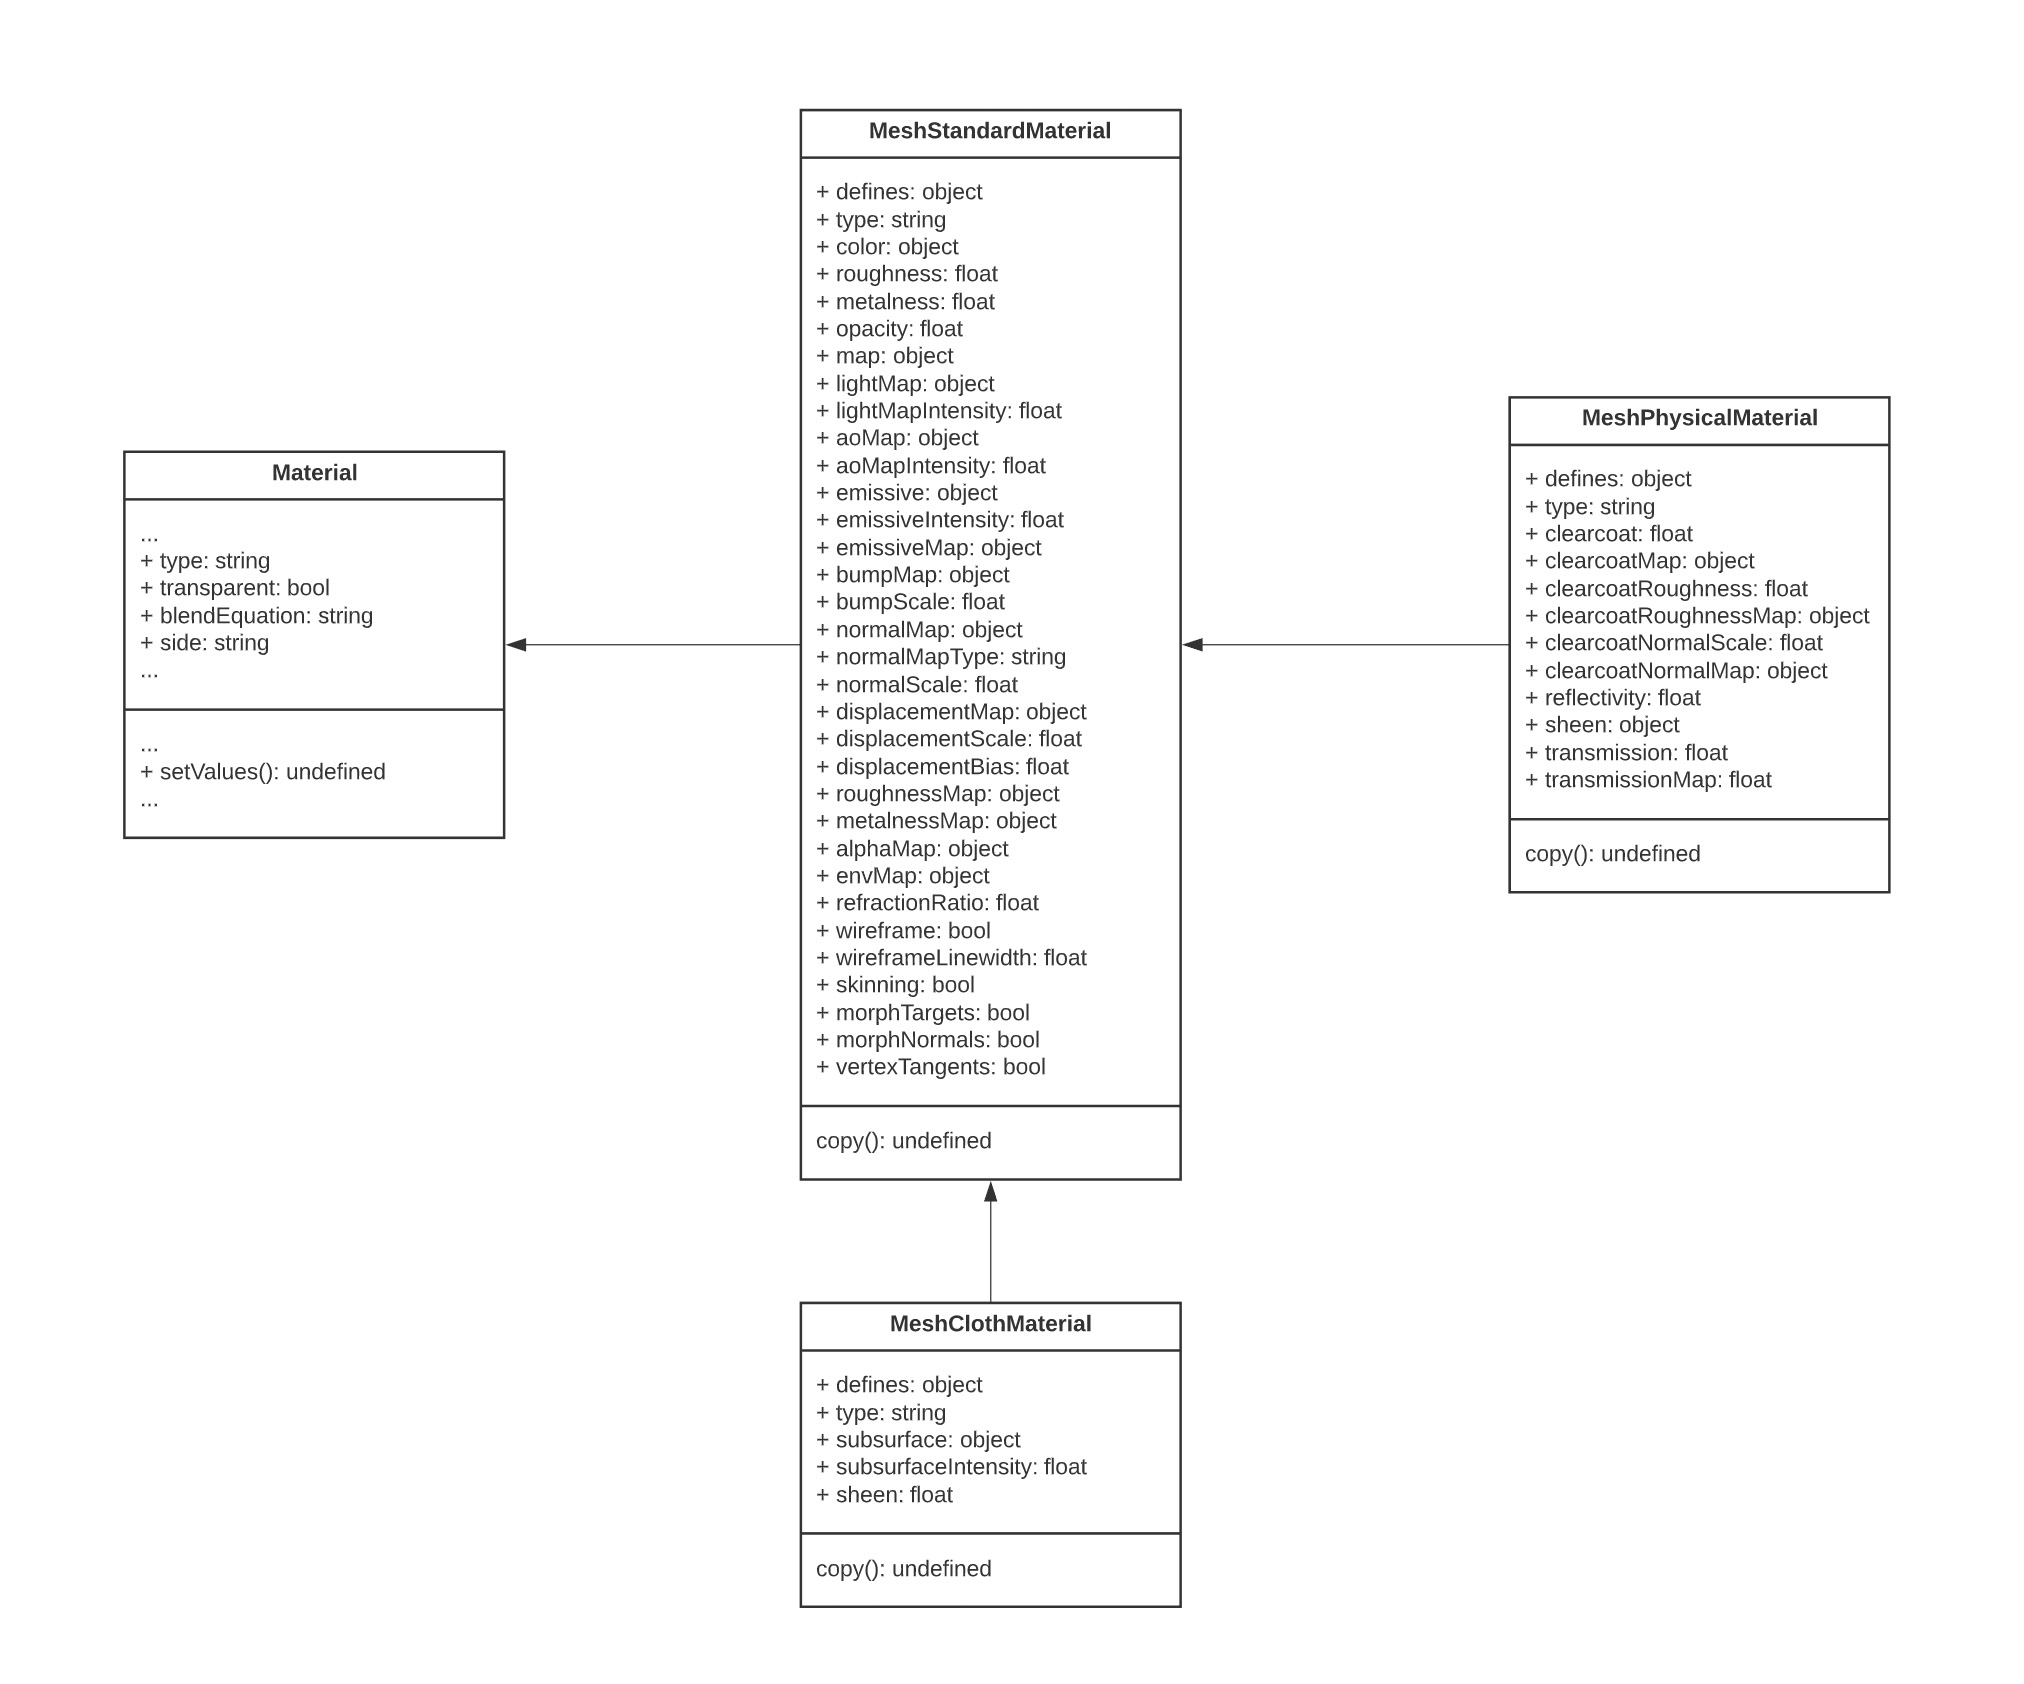
\includegraphics[scale=0.6]{clothschema}}
  \caption{Integraci\'on de la nueva clase \textit{MeshClothMaterial}}
\end{figure}
\singlespacing

El nuevo material tiene un BRDF diferente al \textit{MeshPhysicalMaterial},
y diferentes par\'ametros, sin embargo soporta los mismos efectos de \textit{normal mapping}, \textit{displacement}, etc.
y comparte gran cantidad de los par\'ametros con el material base, a\~nadiendo \textit{subsurface}, \textit{sheen}.
\textit{MeshClothMaterial} utiliza sus propios \textit{type}, para identificar el tipo de shader, en la clase \textit{WebGLMaterials}
y \textit{defines}, que se utilizar\'an para a\~nadir directivas de preprocesador al c\'odigo GLSL generado en la clase
\textit{WebGLProgram}. Para que el nuevo material est\'e expuesto como un material nativo de ThreeJs,
se an\~ade a objeto \textit{Materials}.

\begin{figure}[H]
  \vspace{0.5cm}
  \centering
    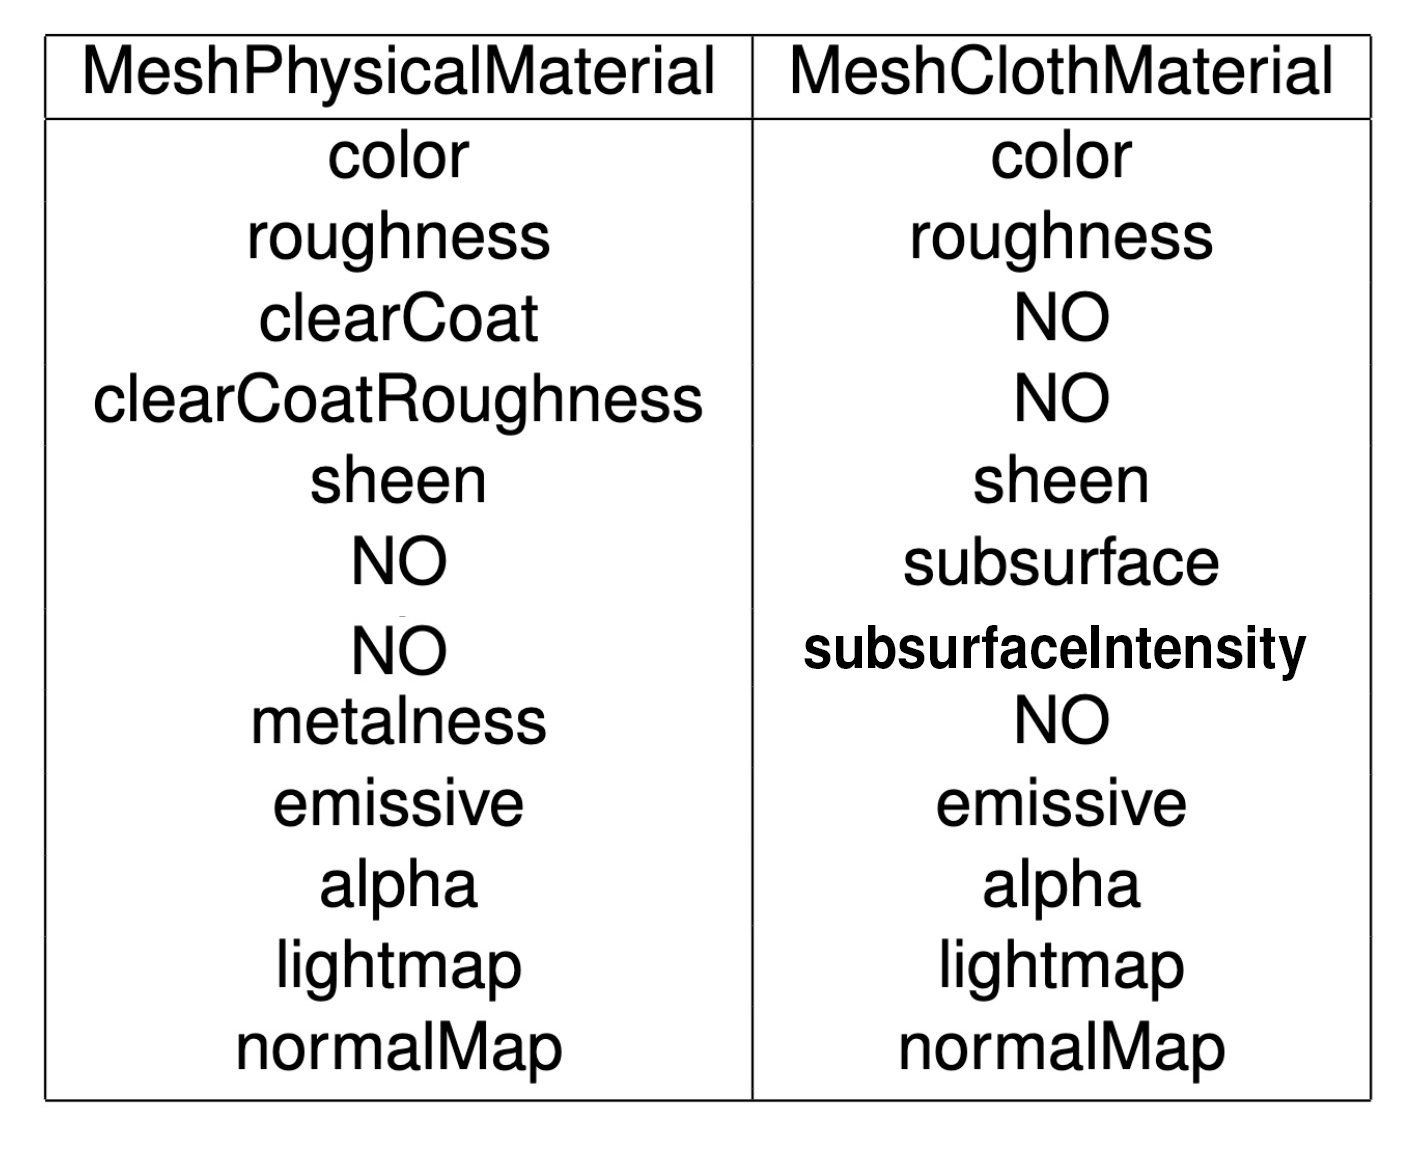
\includegraphics[scale=0.34]{table}
  \caption{Comparativa \textit{MeshPhysicalMaterial}, \textit{MeshClothMaterial}}
\end{figure}


En la clase \textit{WebGLMaterials} se incluye un nuevo m\'etodo para actualizar los par\'ametros de \'este nuevo material.\\

\singlespacing
\begin{lstlisting}[caption=Cambios sobre la clase WebGLMaterials de ThreeJs]
// WebGLMaterials.js

// ...
refreshUniformsCommon( uniforms, material );
// ...
function refreshUniformsCloth( uniforms, material, environment ) {

  refreshUniformsStandard( uniforms, material, environment );

  uniforms.reflectivity.value = material.reflectivity;

  if ( material.sheen ) {

    uniforms.sheen.value.copy( material.sheen );

  } else {

    uniforms.sheen.value.copy( material.color );
    uniforms.sheen.value.r = Math.sqrt( uniforms.sheen.value.r );
    uniforms.sheen.value.g = Math.sqrt( uniforms.sheen.value.g );
    uniforms.sheen.value.b = Math.sqrt( uniforms.sheen.value.b );

  }

  if ( material.subsurface ) {
    uniforms.subsurface.value.copy( material.subsurface );
  }

  if ( material.brdfCloth ) {
    uniforms.brdfCloth.value = material.brdfCloth;
  }
}
// ...
\end{lstlisting}
\singlespacing

En la clase \textit{WebGLProgram} se modifica el constructor para para a\~nadir las directivas de precompilaci\'on
para los par\'ametros \textit{subsurface} y \textit{sheen}, en caso de utilizarse estos par\'ametros.\\

\begin{lstlisting}[caption=Cambios sobre la clase WebGLProgram de ThreeJs]
// WebGLProgram.js
// ...
function WebGLProgram( renderer, cacheKey, parameters, bindingStates ) {
  // ...
  prefixFragment = [
    // ...
    ( parameters.sheen || parameters.shaderID === 'cloth' ) ? '#define USE_SHEEN' : '',
    parameters.subsurface ? '#define SUBSURFACE' : '',
    // ...
  ]
  // ...
}
// ...
\end{lstlisting}
\singlespacing

En \textit{WebGLPrograms} se an\~ade una clave para el nuevo tipo de material, \textit{MeshClothMaterial}
y se a\~naden las cadena de texto \textit{subsurface}, \textit{subsurfaceIntensity} y \textit{sheen} al array \textit{parameterNames}, adem\'as de a\~nadir nuevas claves para
el \textit{subsurface} y \textit{sheen} y la informaci\'on precomputada del BRDF, dentro del objeto \textit{parameters} dentro de la funci\'on
\textit{getParameters}. De esta forma nos aseguramos que el sistema interpreta correctamente el nuevo material y puede acceder
y cachear sus propiedades.

\singlespacing
\begin{lstlisting}[caption=Cambios sobre la clase WebGLPrograms de ThreeJs]
// WebGLPrograms.js
// ...
const shaderIDs = {
  // ...
  MeshClothMaterial: 'cloth',
  // ...
};

const parameterNames = [
  // ...
  "subsurface", "brdfCloth",
  // ...
];
// ...
function getParameters( material, lights, shadows, scene, object ) {
  // ...
  const parameters = {
    // ...
    subsurface: !! material.subsurface,
    brdfCloth: !! envMap && shaderID === 'MeshClothMaterial',
    // ...
  };
  // ...
}
// ...
\end{lstlisting}


% ThreeJs utiliza un sistema de chunks (trozos) se componen en tiempo de ejecuci\'on para acabar formando los vertex
% y fragment shaders que se utilizan en los programas de WebGL. Los chunks se componen en la libreria de shaders, la
% clase ShaderLib.
% Para crear nuestro MeshClothMaterial, hemos de extender de la clase base Material, de la que extienden el resto de
% materiales. En este caso, de la misma forma que hace MeshPhysicalMaterial, extenderemos de MeshStandardMaterial,
% que dispone de la mayor parte de uniforms y attributes que necesita nuestro shader.\\

% Para que el motor de render de ThreeJs reconozca este nuevo material es necesario, a\~nadir
% su tipo (MeshClothMaterial) al mapa de ShaderIds para que el gestor de programas (WebGLPrograms)
% lo utilice para detectar obtener los uniforms y shaders necesarios para el material. Adem\'as
% los nuevos par\'ametros necesarios para el material se deben de incluir en el array
% parametersNames, de forma que el sistema de cacheo de programas de ThreeJs detecte estas
% nuevas propiedades.\\

% Finalmente, en el gestor de materiales de ThreeJs, necesitamos a\~nadir un nuevo m\'etodo
% que actualice los unfiroms del programa creado, de la misma forma que se hace con los
% materiales nativos de la librer\'ia.\\

% De esta forma, tenemos un material con la interfaz nativa de ThreeJs, que tiene acceso a los
% chunks definidos en la clase ShaderChunk y cuyos uniforms y composici\'on de chunks definiremos
% en ShaderLib.\\

% El BRDF para el componente especular de la iluminaci\'on directa del material Cloth de Filament,
% se utiliza en ThreeJs para a\~nadir opcionalmente un l\'obulo de Sheen al material. Por otra
% parte, el difuso, utiliza en Filament un t\'ermino opcional para ofrecer una aproximaci\'on
% barata el subsurface scattering para iluminaci\'on directa que utiliza Filament.\\


\vspace{1cm}
\section{Integraci\'on del nuevo \textit{shader} sobre ThreeJs}
  Para a\~nadir un nuevo BRDF hemos de extender el sistema de \textit{chunks} de ThreeJs. Para ello hemos de a\~nadir el
  punto de entrada del nuevo shader al objeto \textit{shaderChunk}. Siguiendo el sistema de nomenclatura de ThreeJs,
  llamaremos \textit{meshcloth\_frag.glsl.js} al nuevo shader, que utiliza chunks comunes con el \textit{MeshStandardMaterial},
  salvo para el c\'aculo de la iluminaci\'on directa e indirecta, que utiliza sus propios \textit{chunks} para el c\'aculo
  de la ecuaci\'on de render: \textit{lights\_cloth\_fragment.glsl.js}, donde se inicializa la estructura de datos relativa
  al material y \textit{lights\_cloth\_pars\_fragment.glsl.js}, donde se calculan las ecuaciones de render de la iluminaci\'on
  directa e indirecta del nuevo material.

  \subsection{Componente difusa}
  El color difuso y el color de \textit{subsurface}, modelan en realidad el mismo fen\'omeno f\'isico, la cantidad de reflexi\'on
  interna que resulta en aportaci\'on sobre la reflexi\'on en direcci\'on al vector de vista. Cuando la luz absorbida y reflejada
  sale de nuevo por un punto cercano al punto de entrada, el efecto de absorci\'on y reflexi\'on interna es despreciado y se modela como el
  color difuso. Por otra parte, cuando la luz absorbida se emite de nuevo hacia fuera desde un punto diferente al de entrada,
  el efecto se modela como \textit{subsurface scattering}.
  
  El modelo para tejidos de Filament utiliza el difuso de Lambert en caso de no utilizar el par\'ametro \textit{subsurface},
  mientras que si lo utiliza el factor de correcci\'on de la t\'ecnica \textit{wrapped diffuse lighting} \autocite{gpugems}
  que permite aproximar el efecto debido a la absorci\'on y reflexi\'on interna de la luz incidente en la superficie.\\

  \begin{eqfloat}[!htb]
    \begin{equation}
      f_d(v, h) = \frac{c_{diff}}{\pi}
      \Bigg\langle
      \frac{(n\cdot{l})w}{(1+ w)^2}( c_{subsurface} + n \cdot{l} )
      \Bigg\rangle
    \end{equation}
  \caption{Componente difusa del modelo de \textit{Cloth} en Filament}
  \end{eqfloat}

  \singlespacing
  \begin{lstlisting}[caption=Implementaci\'on del BRDF para la componente difusa de \textit{MeshClothMaterial}]
vec3 BRDF_Diffuse_Cloth(
  const in IncidentLight incidentLight,
  const in vec3 viewDir,
  const in vec3 normal,
  const in vec3 diffuseColor
) {

  float dotNL = dot( normal, incidentLight.direction );
  float radiance = RECIPROCAL_PI; // Lambert BRDF
  
  #if defined(SUBSURFACE)
    // Fd_Wrap
    radiance *= saturate(
      (dotNL + subsurfaceIntensity)
      / ((1.0 + subsurfaceIntensity) * (1.0 + subsurfaceIntensity))
    );
  #endif

  vec3 Fd = radiance * diffuseColor;

  return Fd;

}

void RE_Direct_Cloth(
  const in IncidentLight directLight,
  const in GeometricContext geometry,
  const in PhysicalMaterial material,
  inout ReflectedLight reflectedLight
) {

  // ...
  reflectedLight.directDiffuse += irradiance * BRDF_Diffuse_Cloth(
    directLight,
    geometry.viewDir,
    geometry.normal,
    material.diffuseColor
  );

  #if defined(SUBSURFACE)
    reflectedLight.directDiffuse *= saturate(subsurface + dotNL); 
  #endif
  // ...

}
  \end{lstlisting}


  \subsection{Componente especular}

  El \textit{MeshPhysicalMaterial} utiliza por defecto un BRDF GGX, \autocite{ggx}. Sin embargo, si el par\'ametro de \text{sheen}
  est\'a activo, utiliza 
  Al contrario que el MeshPhysicalMaterial, que utiliza una una distribucion GGX, el material
  Cloth de Filament utiliza una versi\'on modificada del BRDF presentado por Ashikmin y Premoze. En la versi\'on de Filament,
  la presentada por \autocite{theordertalk}, se utilizan dos nuevos par\'ametros que permiten control sobre la escala
  y desplazamiento del especular. 

  \autocite{ashikhmin}\\

  \textit{Velvet distribution} \autocite{ashikhmin}:\\

  \begin{equation}
    D_{Velvet}(v, h, \alpha) = c_{norm} (
      1 + 4exp \left(\frac{-cot^2\theta_h}{\alpha^2}\right)
    )
  \end{equation}
  \singlespacing

  Componente difusa del modelo de \textit{Cloth} en Filament:\\

  \begin{equation}
    D_{Charlie}(\alpha) = \frac
    {(2 + \frac{1}{\alpha})sin(\theta)^\frac{1}{\alpha}}
    {2\pi}
  \end{equation}
  \singlespacing

  \begin{lstlisting}[caption=Implementaci\'on del factor de distribuci\'on de Charlie en ThreeJs]
float D_Charlie(float roughness, float NoH) {
  // Estevez and Kulla 2017, "Production Friendly Microfacet Sheen BRDF"
  float invAlpha = 1.0 / roughness;
  float cos2h = NoH * NoH;
  float sin2h = max(1.0 - cos2h, 0.0078125); // 2^(-14/2), so sin2h^2 > 0
                                             // in fp16
  return (2.0 + invAlpha) * pow(sin2h, invAlpha * 0.5) / (2.0 * PI);
}
  \end{lstlisting}
  \singlespacing

  Mientras que para el factor de geometr\'ia o visibilidad se utiliza la version modificada de Neubelt \autocite{theorder}
  del denominador de microfacetas para suavizar el degradado de la sombra.\\

  Formulaci\'on del t\'ermino de geometr\'ia de Neubelt \autocite{theorder}:\\
    
  \begin{equation}
    \frac{1}{4(n\cdot{l} + n\cdot{v} - (n\cdot{l})(n\cdot{v}) )}
  \end{equation}
  \singlespacing

  \begin{lstlisting}[caption=Implementaci\'on del t\'ermino de de visibilidad de Neubelt \autocite{theorder}]
float V_Neubelt(float NoV, float NoL) {
  // Neubelt and Pettineo 2013, "Crafting a Next-gen Material Pipeline for The Order: 1886"
  return saturate(1.0 / (4.0 * (NoL + NoV - NoL * NoV)));
}
  \end{lstlisting}

  \singlespacing
  \begin{lstlisting}[caption=Cambios sobre la clase WebGLPrograms de ThreeJs]
vec3 BRDF_Specular_Sheen( const in float roughness, const in vec3 L, const in GeometricContext geometry, vec3 specularColor ) {

  vec3 N = geometry.normal;
  vec3 V = geometry.viewDir;

  vec3 H = normalize( V + L );
  float dotNH = saturate( dot( N, H ) );

  return specularColor * D_Charlie( roughness, dotNH ) * V_Neubelt( dot(N, V), dot(N, L) );

}
  \end{lstlisting}

  \subsection{Iluminaci\'on indirecta}
    De las t\'ecnicas de iluminaci\'on indirecta vistas en el cap\'itulo 3, ThreeJs soporta tanto mapas de
    irradiancia como esf\'ericos harm\'onicos para la componente difusa, mientras que para la componente
    especular utiliza la aproximaci\'on anal\'itica presentada por Lazarov \autocite{blackops}.

    \subsubsection{Componente difusa}
      Para el c\'alculo del difuso, ha de estimarse la irradiancia debida al entorno sobre un punto y multiplicarlo
      por el BRDF difuso. ThreeJs soporta ambas t\'enicas vistas en el cap\'itulo 3 para el c\'alculo de irradiancia:
      mapas de irradiancia y esf\'ericos harm\'onicos.

      C\'alculo de la luz indirecta difusa: \\

      \begin{equation}
        L_o(p, w_o) = k_d \frac{c}{\pi} \int_{\Omega}{L_i(p, w_i) n\cdot{w_i}dw_i}
      \end{equation}
      \singlespacing

      Los \textit{chunks} de ThreeJs separan el c\'aculo de la luz indirecta en una funci\'on para cada componente, difuso
      y especular. El c\'aculo de la componente difusa se realiza en la funci\'on \textit{RE\_IndirectDiffuse\_Cloth}.\\

      \begin{lstlisting}[caption=C\'alculo de la ecuaci\'on de render para la componente difusa de \textit{MeshClothMaterial}]
  void RE_IndirectDiffuse_Cloth( const in vec3 irradiance, const in GeometricContext geometry, const in PhysicalMaterial material, inout ReflectedLight reflectedLight ) {
  
      reflectedLight.indirectDiffuse += irradiance * BRDF_Diffuse_Lambert( material.diffuseColor );
  
  }
      \end{lstlisting}

      Sin embargo, para tener en cuenta el principio de conservaci\'on de la energ\'ia, $k_d + k_s = 1$, tal y como se
      presenta en el modelo de Cook-Torrance \autocite{cooktorrance}, parte del c\'alculo se hace en la funci\'on
      \textit{RE\_IndirectSpecular\_Cloth}, que eval\'ua la componente especuar. \textit{RE\_IndirectSpecular\_Cloth}
      utiliza un mapa prefiltrado de entorno, explicado en el cap\'itulo 3, para calcular la irradiancia, que se le resta al
      total de energ\'ia (1), para obtener el peso de la irradiancia difusa. Finalmente, en caso de utilizar \textit{subsurface},
      se aplica el factor de correcci\'on.\\



      % ThreeJs utiliza dos enfoques, por una parte, mapas de irradiancia y por otra, light probes, que
      % utilizan spherical harmonics. Los mapas de irradiancia son una tecnica IBL (Image Based Lighting)
      % tratan todo el entorno como una fuente de luz y utilizan im\'agenes precomputadas que permiten
      % acelerar este calculo.\\

      % La parte integral de la ecuaci\'on se resuelve utilizando el mapa de irradiancia,
      % que utiliza un factor de correci\'on en caso de estar modelando la refracci\'on interna,

      \begin{lstlisting}[caption=Conservaci\'on de la energ\'ia y \textit{wrapped diffuse lightning} aplicados en la funci\'on de luz indirecta especular]
void RE_IndirectSpecular_Cloth(
  const in vec3 radiance,
  const in vec3 irradiance,
  const in vec3 clearcoatRadiance,
  const in GeometricContext geometry,
  const in PhysicalMaterial material,
  inout ReflectedLight reflectedLight
) {
  // ...

  float diffuseWrapFactor = 1.0;
  #if defined(SUBSURFACE)
    diffuseWrapFactor *= saturate(
      (dotNV + subsurfaceIntensity)
      / ((1.0 + subsurfaceIntensity) * (1.0 + subsurfaceIntensity))
    );
  #endif

  // E = specular irradiance
  vec3 FdSH = reflectedLight.indirectDiffuse * ( 1.0 - E )
    * diffuseWrapFactor;
  vec3 FdIM = irradiance * BRDF_Diffuse_Lambert( material.diffuseColor )
    * ( 1.0 - E ) * diffuseWrapFactor;

  vec3 Fd = Fd_SH + Fd_Lod;

  #if defined(SUBSURFACE)

    Fd *= saturate(subsurface + dotNV);

  #endif
  // ...

  reflectedLight.indirectDiffuse = Fd;

}
      \end{lstlisting}

      \singlespacing

    \subsubsection{Componente especular}
      Tanto ThreeJs como Filament utilizan la t\'ecnica \textit{split-sum approximation} \autocite{dfgapproximation}
      en la componente especular. Sin embargo, mientras que Filament utiliza un \textit{BRDF integration map},
      ThreeJs utiliza la aproximaci\'on presentada por Epic \autocite{dfgapproximation}, ambas presentadas en
      el cap\'itulo 3.\\

      % \begin{eqfloat}[ht]
      %   \begin{equation}
      %     \resizebox{0.95\hsize}{!}{%
      %     $L_o(p, w_o) =
      %     \int_{\Omega} k_s \frac{DFG}{4(w_o\cdot{n})(w_i\cdot{n})})L_i(p, w_i)n\cdot{w_i}dw_i = \\
      %     \int_{\Omega} k_s \frac{DFG}{4(w_o\cdot{n})(w_i\cdot{n})}) *
      %     \int_{\Omega}L_i(p, w_i)n\cdot{w_i}dw_i$   
      %     }
      %   \end{equation}
      % \caption{Separaci\'on de la integral de la componente especular en la integral del BRDF y la integral de la radiancia }
      % \end{eqfloat}
      
      La aproximaci\'on de ThreeJs del BRDF especular funciona especialmente bien para dispositivos con un rendimiento
      limitado. Esta aproximaci\'on de la integral del BRDF es una soluci\'on anal\'itica para el BRDF GGX \autocite{ggx},
      por lo que no es correcta para el nuevo BRDF del modelo de telas.\\

      \begin{lstlisting}[caption=Apromixaci\'on anal\'itica a la integral del BRDF en ThreeJs]
        vec2 integrateSpecularBRDF( const in float dotNV, const in float roughness ) {
          const vec4 c0 = vec4( - 1, - 0.0275, - 0.572, 0.022 );
          const vec4 c1 = vec4( 1, 0.0425, 1.04, - 0.04 );
          vec4 r = roughness * c0 + c1;
          float a004 = min( r.x * r.x, exp2( - 9.28 * dotNV ) ) * r.x + r.y;
          return vec2( -1.04, 1.04 ) * a004 + r.zw;
        }
      \end{lstlisting}
      \singlespacing
      

      El nuevo modelo de telas, de la misma forma que Filament, utiliza un \textit{BRDF integration map} para almacenar
      en los canales rojo y azul la escala y offset del Fresnel para el modelo GGX \autocite{ggx}. El resultado del BRDF de tejidos,
      que no utiliza Fresnel, se almacena en el canal azul, al que se accede de igual forma que al \textit{BRDF integration map} para el modelo GGX \autocite{ggx},
      utilizando $n\cdot{l}$ para el eje $x$ y el valor de rugosidad del material para el eje $y$.

      % Mientras que Filament utiliza un 

      % Para el especular, la 
      % \autocite{blackops}. \'Esta t\'ecnica permite separar la en dos partes la soluci\'on de la
      % integral.

      % Por una parte, el mapa prefiltrado de entorno es un mapa preconvolucionado que tiene en cuenta
      % los posibles valores de rugosidad del material de forma que a medida que el ruido es mayor, las
      % reflexiones son de un color menos definido. Esta tecnica utiliza simplifica el calculo de
      % la integral asumiendo la direccion de la vista igual a la direccion de sampleo.\\

      % Por otra parte, el c\'alculo del BRDF se almacena en una textura, conocida como mapa de integral
      % del BRDF, utilizando $n\cdot{w_i}$ en el eje $x$ y $roughness$ en el eje y.

      \begin{figure}[H]
        \vspace{0.5cm}
        \centering
          \frame{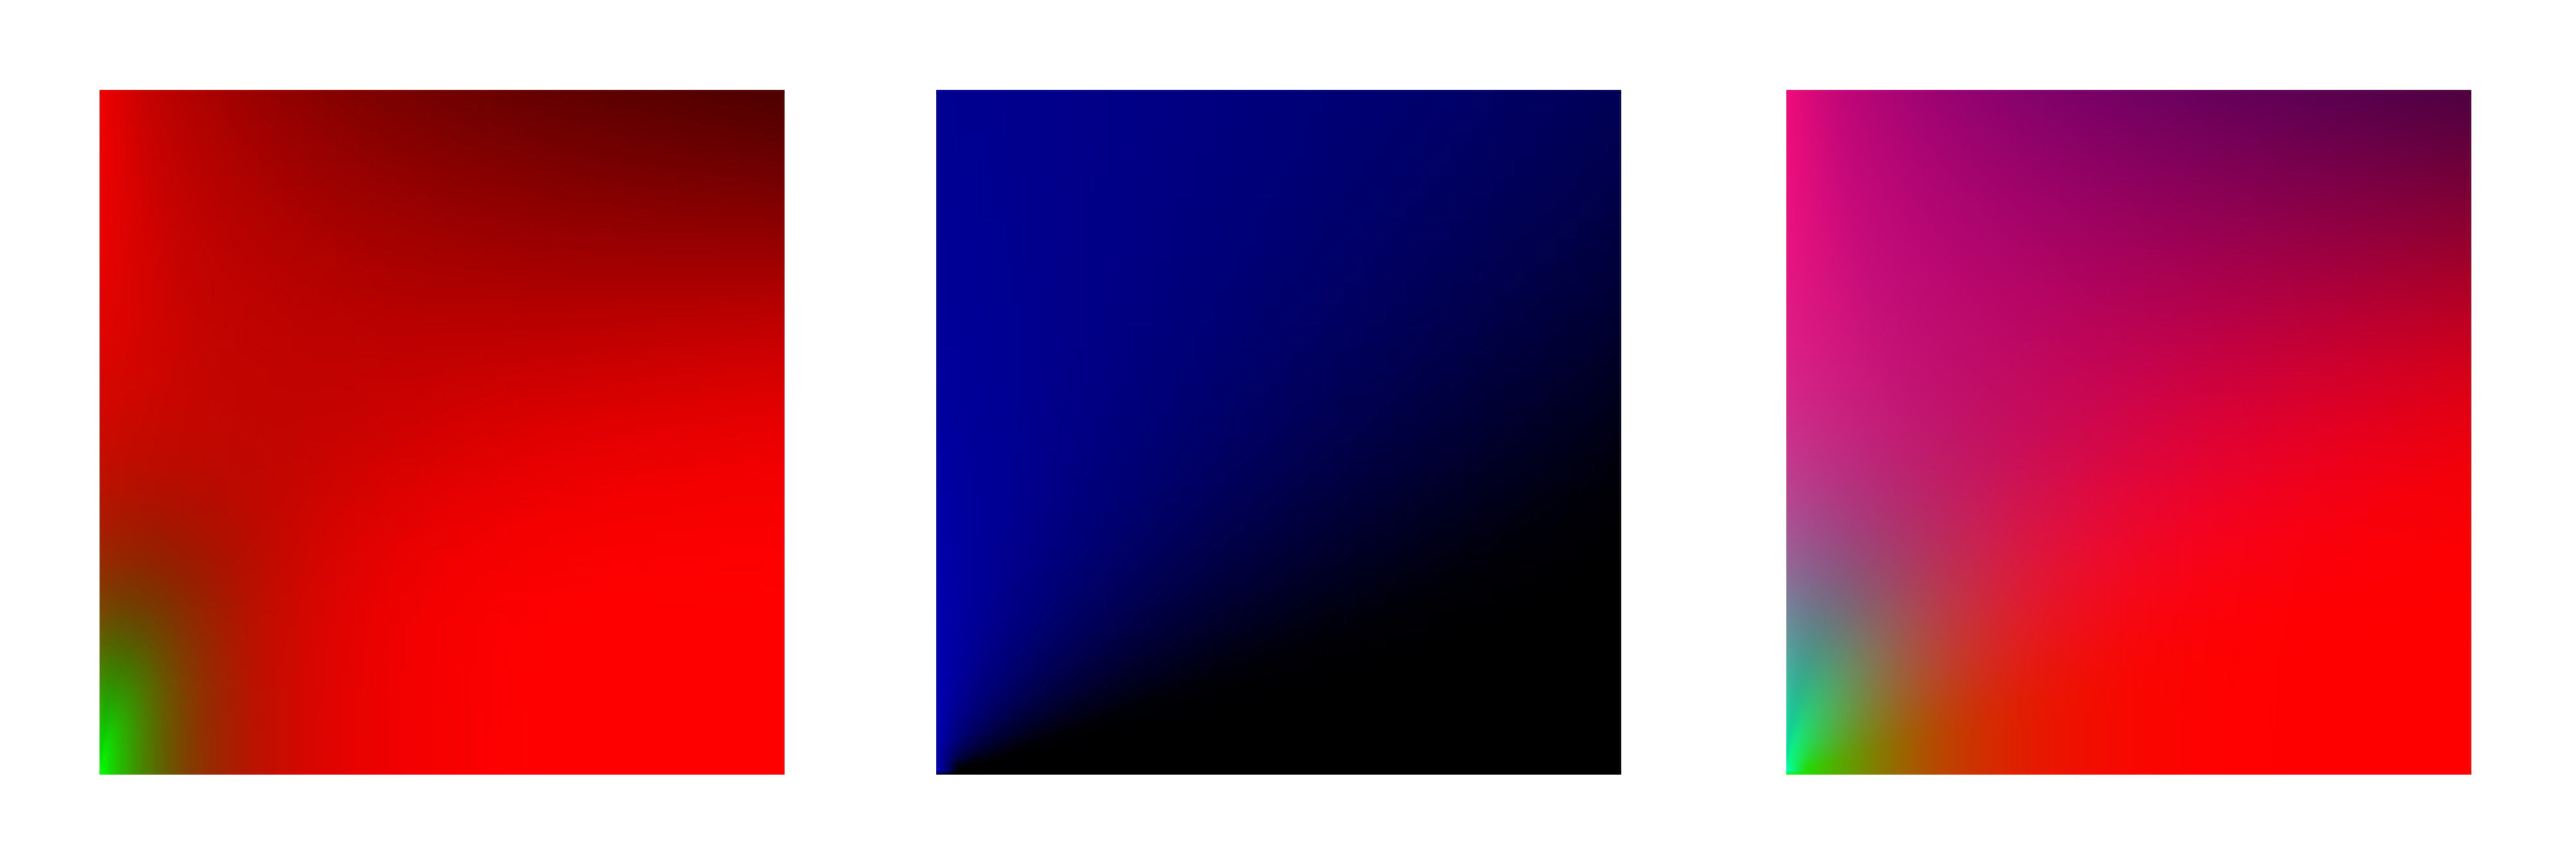
\includegraphics[scale=0.35]{splitsumcloth}}
        \caption{Canales RG (BRDF GGX \autocite{ggx}), B (BRDF para telas \autocite{filament}) y la suma de ellos,
        RGB, del \textit{BRDF integration map}}
        \vspace{0.5cm}
      \end{figure}

    \begin{lstlisting}[caption=C\'alculo de la irradiancia del entorno para el modelo de telas utilizando el nuevo \textit{BRDF integration map}]
float prefilteredDG = textureLod(
  brdfCloth,
  vec2( dotNV, material.specularRoughness * material.specularRoughness ),
  0.0
).b;

vec3 E = material.sheenColor * prefilteredDG;
reflectedLight.indirectSpecular += E * radiance;
    \end{lstlisting}
    \singlespacing

    \begin{lstlisting}[caption=C\'alculo de iluminaci\'on indirecta especular de \textit{MeshClothMaterial}]
void RE_IndirectSpecular_Cloth(
  const in vec3 radiance,
  const in vec3 irradiance,
  const in vec3 clearcoatRadiance,
  const in GeometricContext geometry,
  const in PhysicalMaterial material,
  inout ReflectedLight reflectedLight
) {

  float dotNV = dot( geometry.normal, geometry.viewDir );

  float prefilteredDG = textureLod(
    brdfCloth,
    vec2(
      dotNV,
      material.specularRoughness * material.specularRoughness
    ),
    0.0
  ).b;

  vec3 E = material.sheenColor * prefilteredDG;
  reflectedLight.indirectSpecular += E * radiance;

  // ...

}
    \end{lstlisting}
    \singlespacing

Como res\'umen, la implementaci\'on completa de la luz indirecta para el \textit{MeshClothMaterial}:\\

    \begin{lstlisting}[caption=C\'alculo de las componentes difusa y especular en \textit{MeshClothMaterial}]
void RE_IndirectDiffuse_Cloth( const in vec3 irradiance, const in GeometricContext geometry, const in PhysicalMaterial material, inout ReflectedLight reflectedLight ) {

    reflectedLight.indirectDiffuse += irradiance * BRDF_Diffuse_Lambert( material.diffuseColor );

}

void RE_IndirectSpecular_Cloth( const in vec3 radiance, const in vec3 irradiance, const in vec3 clearcoatRadiance, const in GeometricContext geometry, const in PhysicalMaterial material, inout ReflectedLight reflectedLight) {

  float dotNV = dot( geometry.normal, geometry.viewDir );

  float prefilteredDG = textureLod(brdfCloth, vec2( dotNV, material.specularRoughness * material.specularRoughness ), 0.0).b;
  vec3 E = material.sheenColor * prefilteredDG;
  reflectedLight.indirectSpecular += E * radiance;

  float diffuseWrapFactor = 1.0;
  #if defined(SUBSURFACE)
    diffuseWrapFactor *= saturate((dotNV + subsurfaceIntensity) / ((1.0 + subsurfaceIntensity) * (1.0 + subsurfaceIntensity) ));
  #endif

  // Combine envmap and SH diffuse irradiance
  vec3 Fd_SH = reflectedLight.indirectDiffuse * ( 1.0 - E ) * diffuseWrapFactor;
  vec3 Fd_Lod = irradiance * BRDF_Diffuse_Lambert( material.diffuseColor )  * ( 1.0 - E ) * diffuseWrapFactor;
  vec3 Fd = Fd_SH + Fd_Lod;

  #if defined(SUBSURFACE)

    Fd *= saturate(subsurface + dotNV);

  #endif

  reflectedLight.indirectDiffuse = Fd;

}
    \end{lstlisting}
    \singlespacing

\section{Resultados}

A continuaci\'on se muestran y comentan las im\'agenes como resultado de la implementaci\'on del \textit{MeshClothMaterial}. Los resultados se centran
en el an\'alisis de las citadas propiedades \textit{sheen} y \textit{subsurface}.
% Por una parte se muestran interpolaciones de dichas propiedades frente a un color base constante y por otra,

\begin{figure}[H]
  \vspace{0.5cm}
  \centering
    \frame{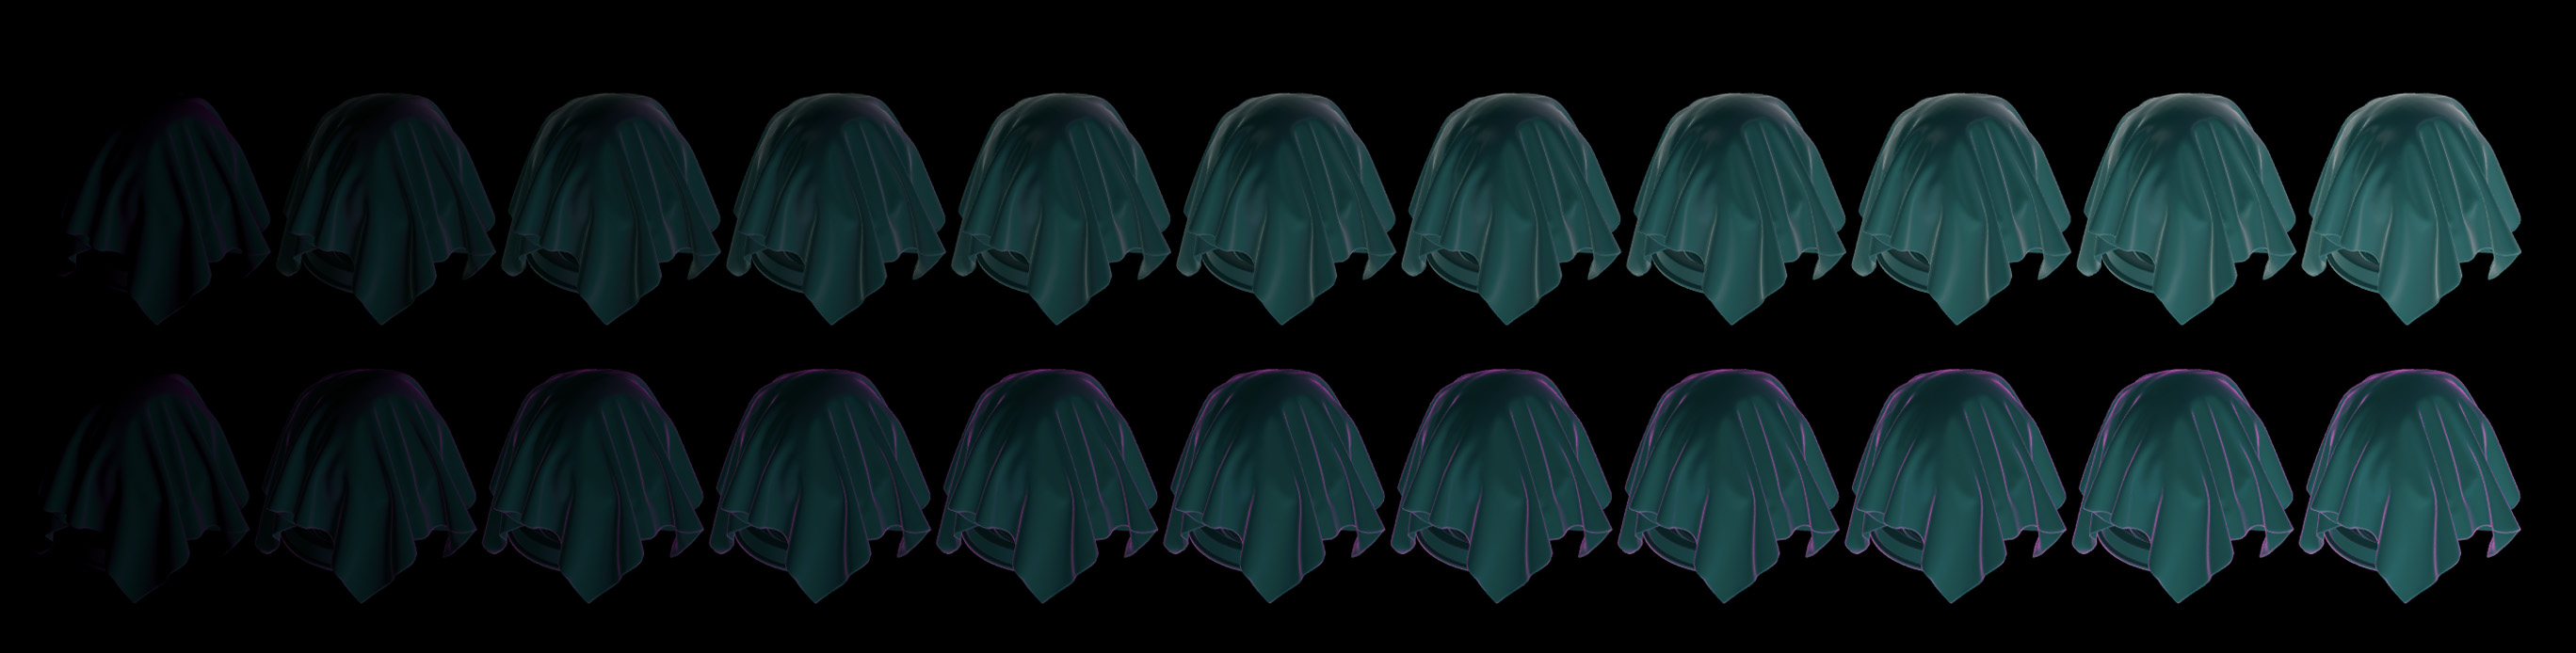
\includegraphics[scale=0.3]{results/ok_cloth_vs_physical.jpg}}
  \caption{Comparativa \textit{MeshPhysicalMaterial} (fila superior) contra \textit{MeshClothMaterial} (fila inferior) incrementando
  progresivamente la intensidad de luz global}
\end{figure}

En la figura 5.4 se muestra una escena en la que la intesidad del la luz de entorno incrementa de izquierda a derecha
frente a una luz direccional muy tenue. El \textit{sheen} de \textit{MeshPhysicalMaterial} solo est\'a soportado en la
iluminaci\'on directa, mientras que para la iluminaci\'on indirecta utiliza la aproximaci\'on anal\'itica del l\'obulo primario.
En la comparativa se muestra como el material de ThreeJs pierde el efecto de \textit{sheen} a medida que aumenta la intesidad
del mapa de entorno. Adem\'as, al utilizar un bajo de rugosidad se hace patente la inconsistencia entre los dos modelos de BRDF
utilizados para la reflexi\'on especular en el \textit{MeshPhysicalMaterial} generando un efecto parecido al de \textit{clearcoat}.


% Utilizando iluminaci\'on indirecta se aprecia que adem\'as de perderse el efecto de \textit{sheen}, las inconsistencia
% entre el BRDF de luz indirecta y el de luz directa cre

\begin{figure}[H]
  \vspace{0.5cm}
  \centering
    \frame{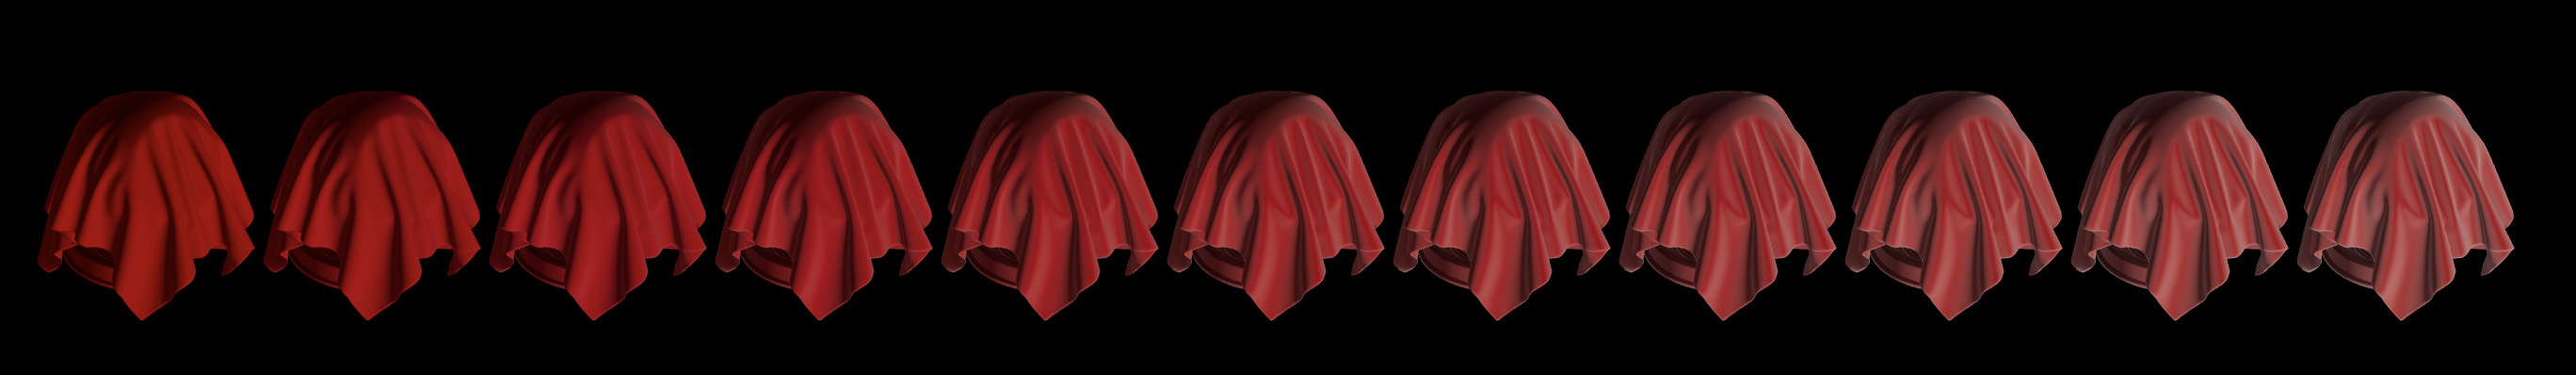
\includegraphics[scale=0.3]{results/ok_sheenintensity.jpg}}
  \caption{Interpolaci\'on de un color de \textit{sheen} aumentando su luminosidad frente a un color base constante.}
\end{figure}

El nuevo material no ofrece un control directo sobre la intensidad del \textit{sheen}, sin embargo, un efecto similar se puede
alcanzar utilizando un el mismo que el color base aumentando la luminosidad como se muestra en la figura 5.5.

\begin{figure}[H]
  \vspace{0.5cm}
  \centering
    \frame{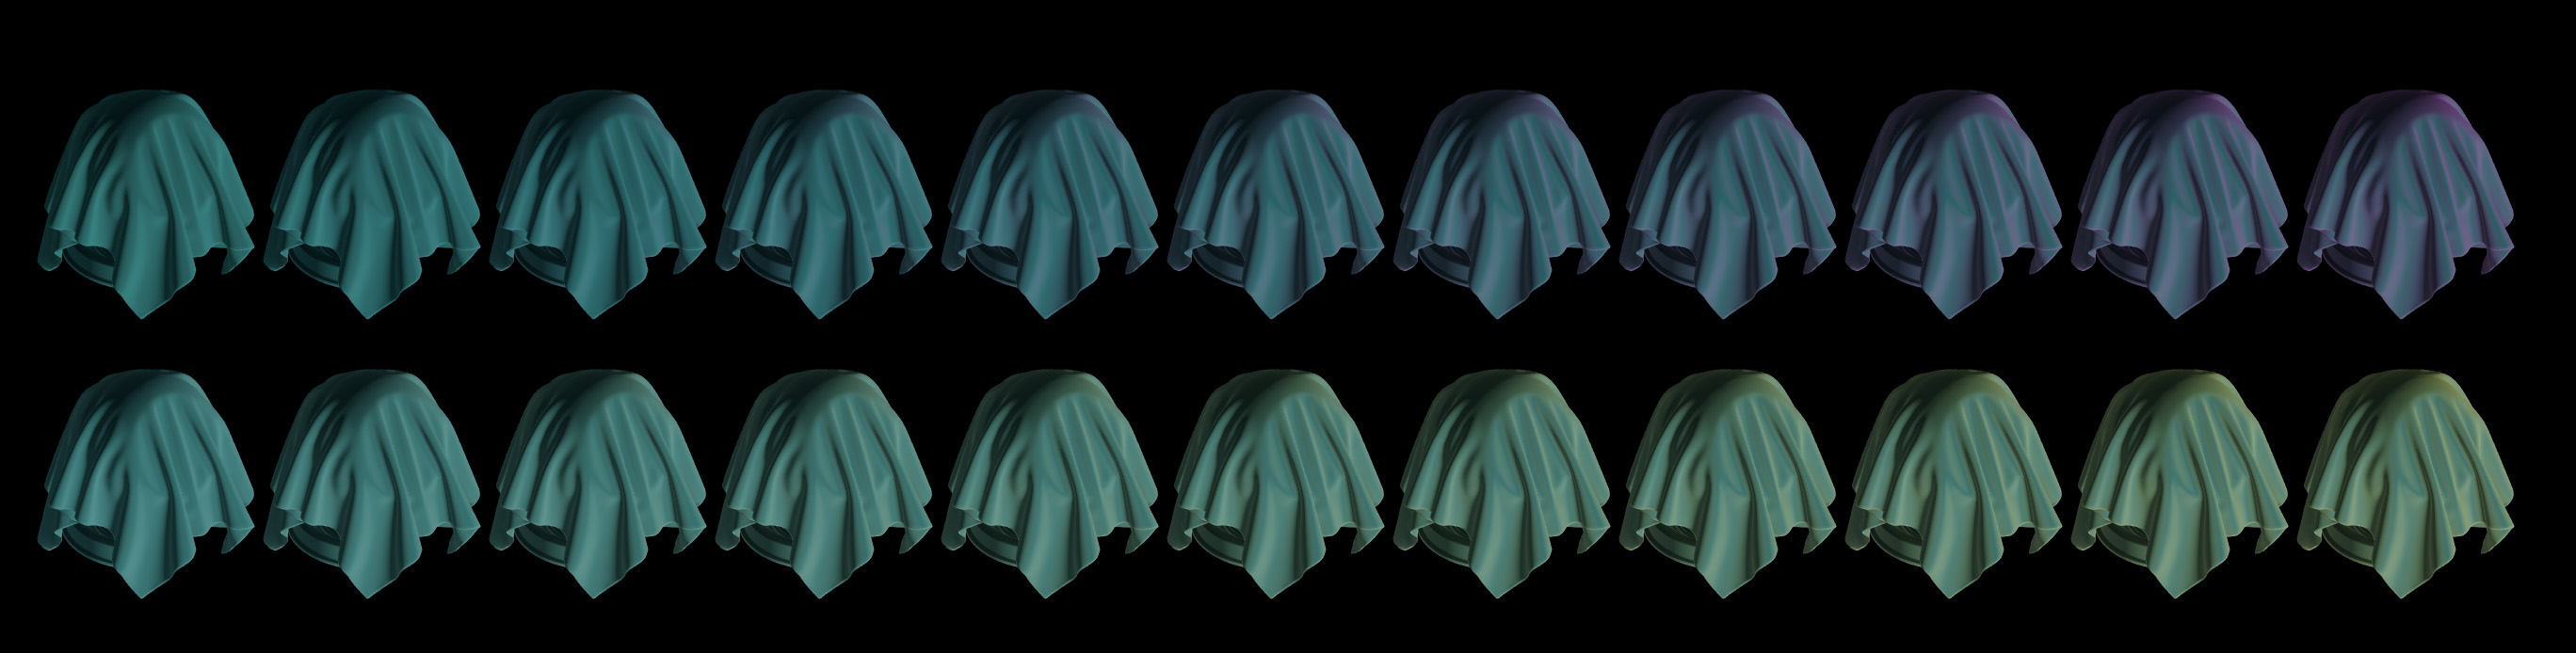
\includegraphics[scale=0.3]{results/ok_sheentint.jpg}}
  \caption{Interpolaci\'on de un color de \textit{sheen} aumentando su saturacion frente a un color base constante.}
\end{figure}
\singlespacing

Como se muestra en la figura 5.6, utilizar un color de \textit{sheen} diferente al color base que, a medida que incrementa su intensidad,
ti\~ne gradualmente el color base a medida que aumenta su saturaci\'on.

\begin{figure}[H]
  \vspace{0.5cm}
  \centering
    \frame{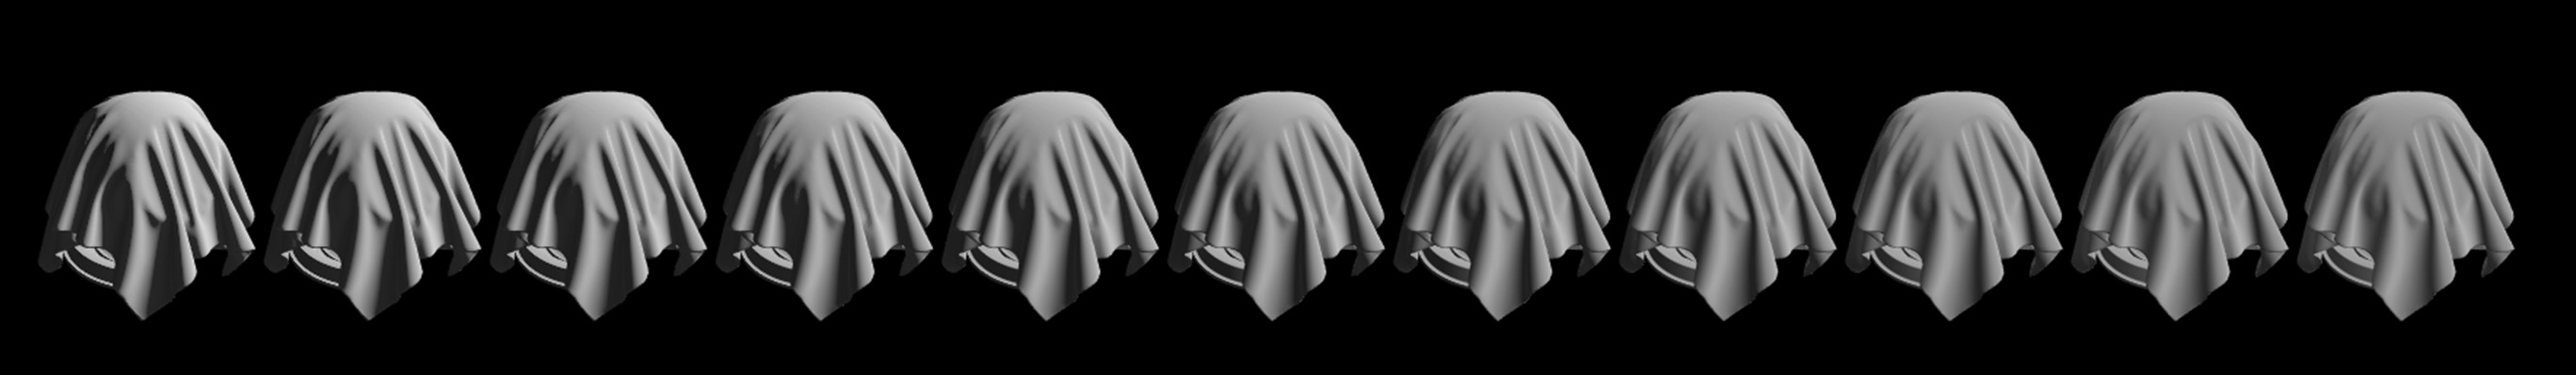
\includegraphics[scale=0.3]{results/ok_subsurfaceintensity.jpg}}
    \caption{Interpolaci\'on de \textit{subsurfaceIntensity} utilizando un color base y color de \textit{subsurface} blancos.}
\end{figure}
\singlespacing

En la figura 5.8, se utiliza el blanco como color base y \textit{subsurface}. La interpolaci\'on del par\'ametro de \textit{subsurfaceIntensity}
muestra una transici\'on de sombras m\'as intensas (\textit{subsurfaceIntensity = 0}) a sombras m\'as suaves, que toman el color base del
\textit{subsurface} (\textit{subsurfaceIntensity = 1})\\

% el color base permanece constante, mientras que el \textit{subsurface}, de un tono similar al color base,
% aumenta su saturaci\'on. Del mismo modo que en el \textit{sheen}, jugando con el valor de luminosidad del \textit{subsurface},
% se puede obtener control sobre la intensidad del efecto.


\begin{figure}[H]
  \vspace{0.5cm}
  \centering
    \frame{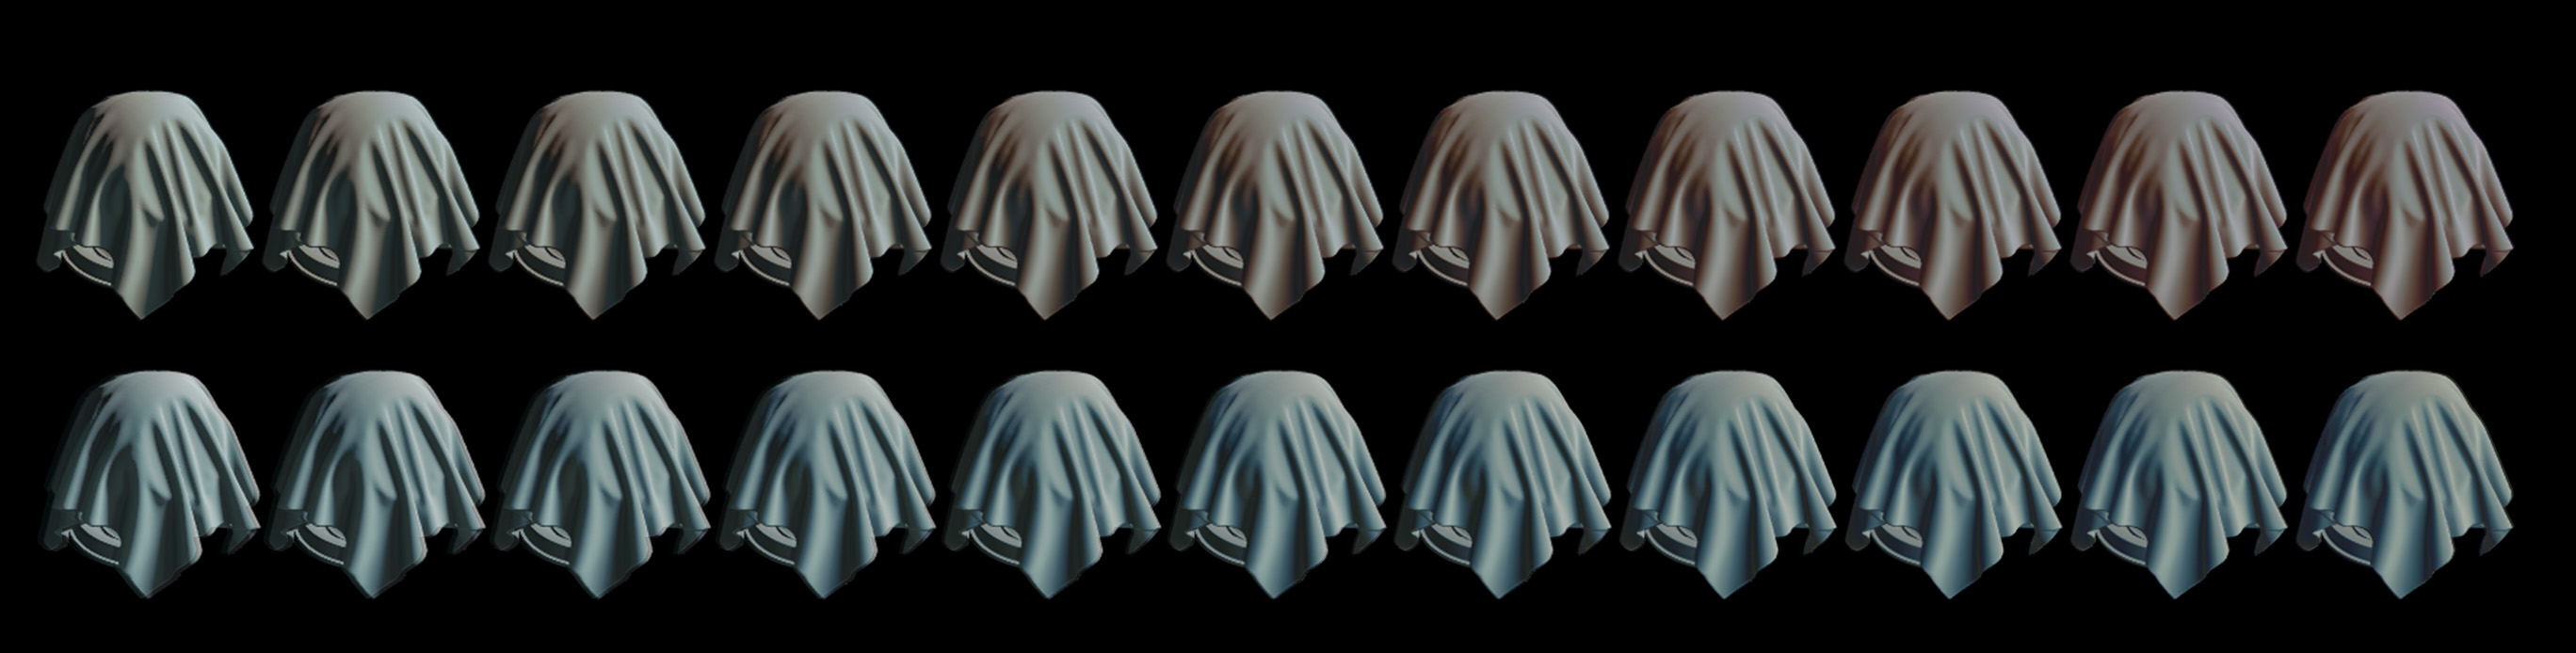
\includegraphics[scale=0.3]{results/ok_subsurfacetint.jpg}}
    \caption{Interpolaci\'on de un color de \textit{subsurface} frennte a un color base constante.}
 \end{figure}
\singlespacing

La figura 5.7 muestra interpolaciones entre un color base constante (blanco) y un color de \textit{subsurface},
rojo en la fila superior y azul en la fila inferior. Subiendo el valor de \textit{subsurfaceIntensity}
se puede apreciar como el tejido se ti\~ne progresivamente del color de \textit{subsurface}.

% se utilizan dos tonos de color complementarios para el color base y el \textit{subsurface}. El color
% base es constante, mientras que el \textit{sheen} aumenta por pasos su saturaci\'on.
% El factor de correcci\'on aplicado sobre el color difuso, que simula el efecto de reflexi\'on interna, ti\~ne progresivasivamente
% las sombras del color asignado al par\'ametro \textit{subsurface}.

% Las siguientes comparativas son matrices bidimensionales que muestran la evoluci\'on de un par\'ametro por cada uno de los ejes
% $x$ e $y$ y permiten ver la relaci\'on entre estos dos par\'ametros y su efecto sobre la apariencia final del material.\\

% En la comparativa de la figura 6.7, se muestra en el eje $x$ un aumento del efecto de \textit{sheen}, mientras que en el
% eje $y$ aumenta el valor de roughness del material. Se puede apreciar que con valores bajos de \textit{sheen}, el efecto
% se aprecia con intensidad en los \'angulos cr\'iticos y decae r\'apidamente, mientras que para valores altos de este par\'ametro,
% el efecto se extiende hacia los tonos medios, creando una transici\'on m\'as suave entre el color base y el de \textit{sheen}.\\

% La figura 6.8 muestra los incrementos del color de \textit{sheen} en el eje $x$ e incrementos en el eje $y$ del color de subsurface.
% El \textit{sheen} de color verde simula el efecto de retrodispersi\'on que ti\~ne el brillo especular de \'este color, mientras
% que el \textit{subsurface}, de color rojo, da a los tonos medios un color rojizo. El valor de \textit{roughness} del material
% es alto, es por ello que a medida que aumentan los valores de \textit{subsuface}, \textit{sheen}, se aprecia una transici\'on
% suave entre estos dos par\'ametros, que proporcionan el aspecto amarillo/anaranjado, como resultado de la transici\'on entre
% el verde del brillo especular y el rojo de las sombras y tonos medios.

\begin{figure}[H]
  \vspace{0.5cm}
  \centering
    \frame{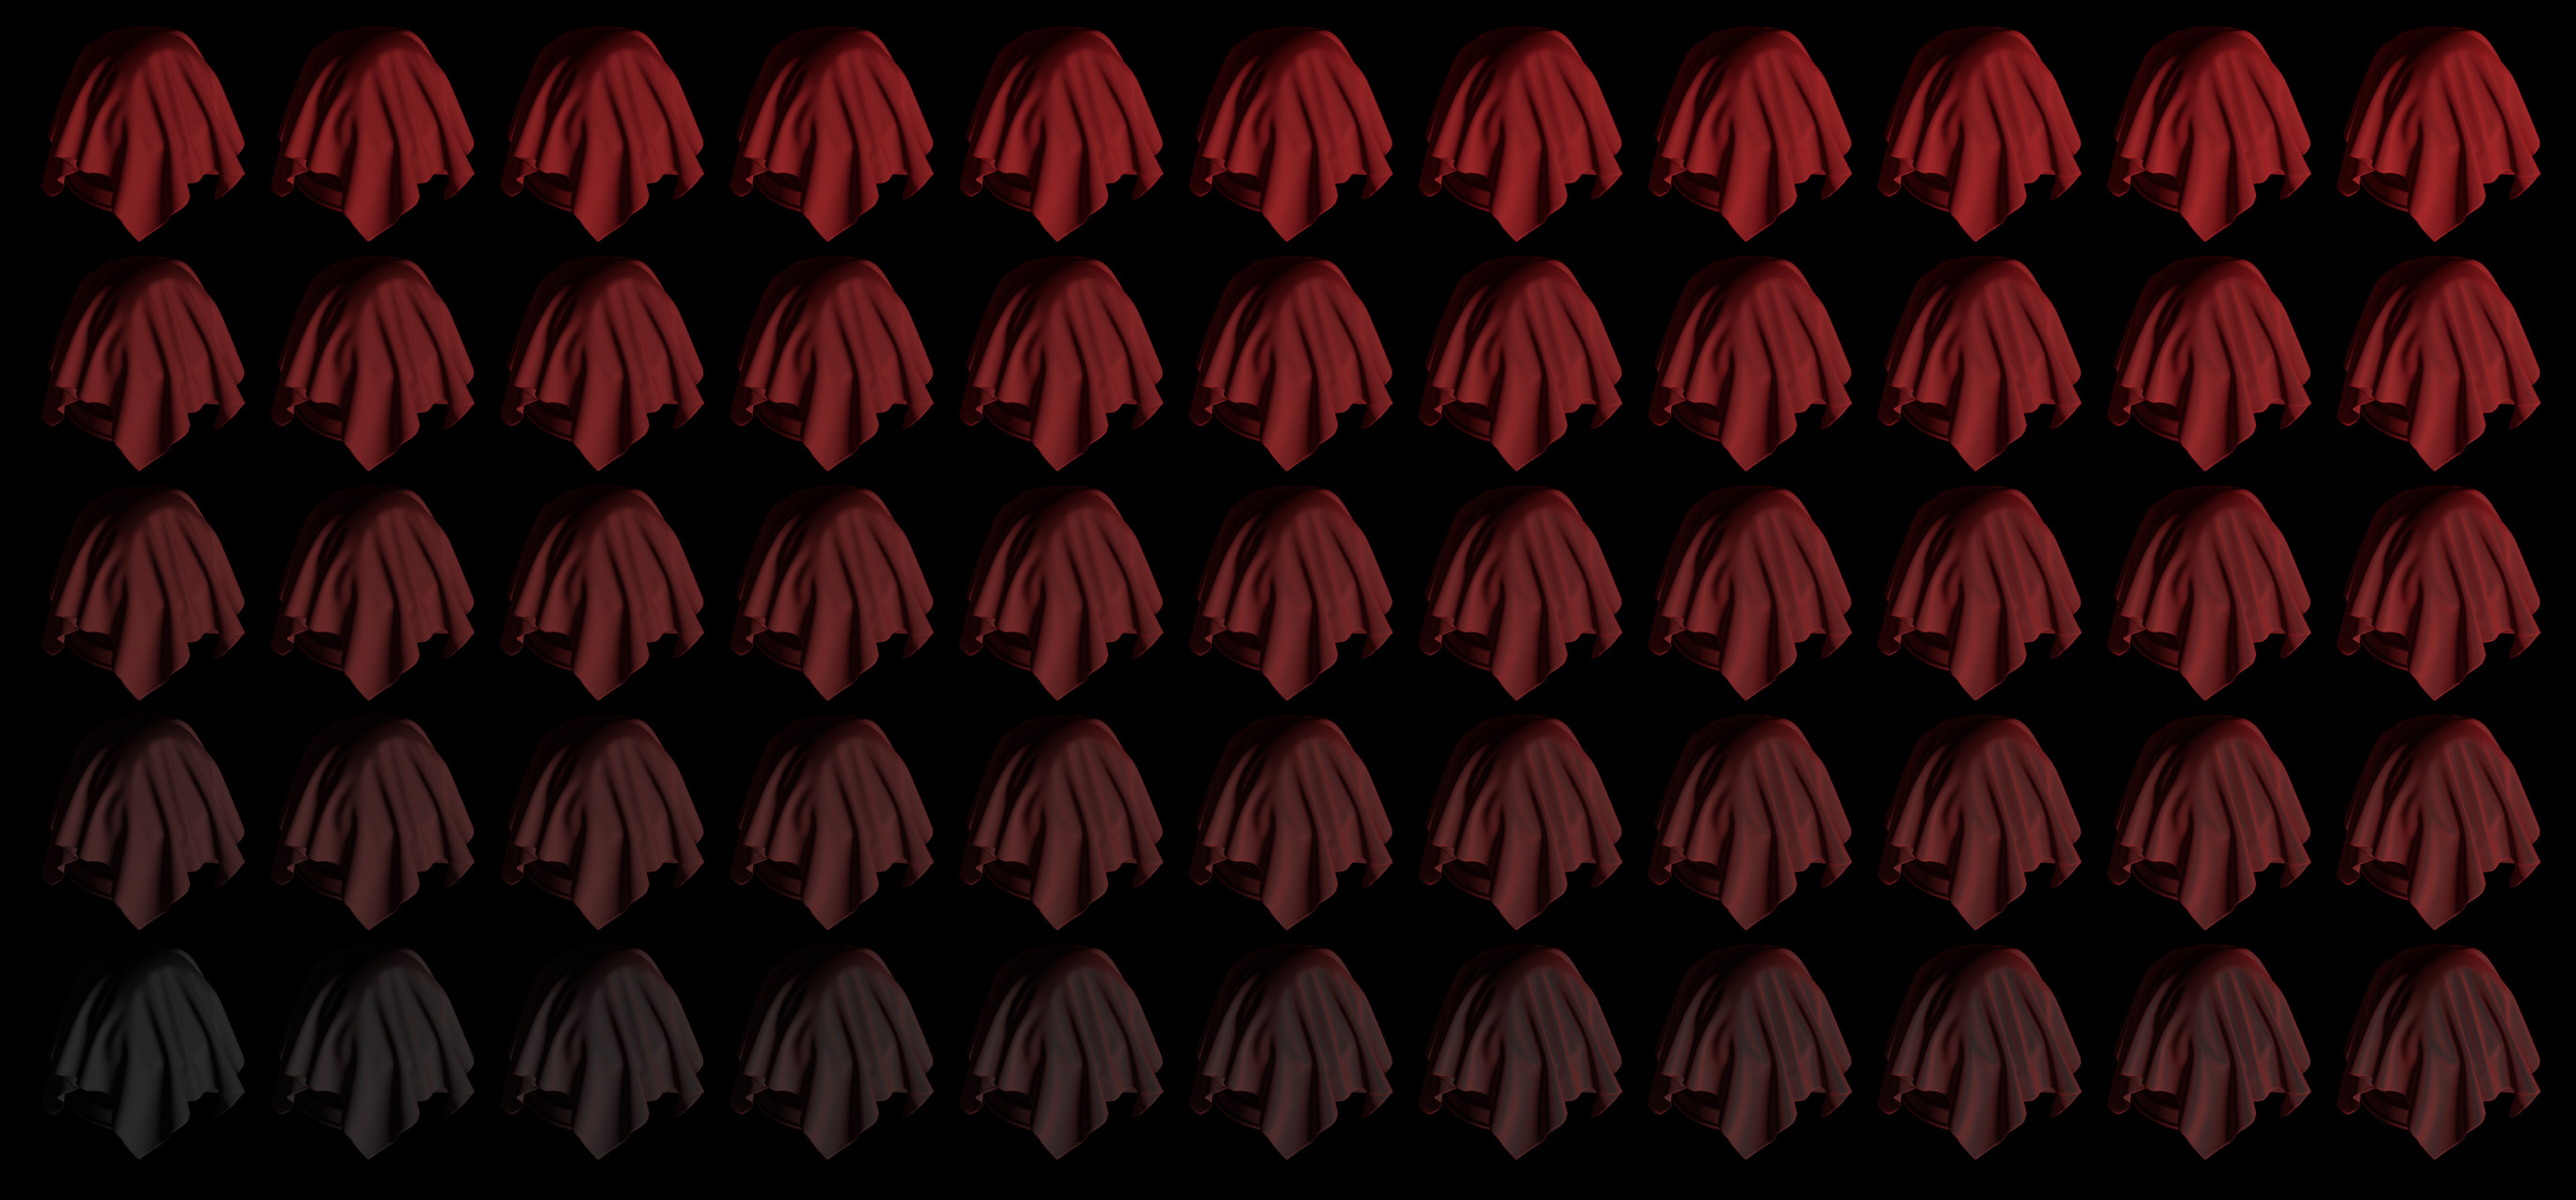
\includegraphics[scale=0.3]{results/ok_basecolorsheen.jpg}}
    \caption{Interpolaci\'on del color de sheen en el eje $x$ frente a interpolaci\'on del color base en el eje $y$.}
\end{figure}

La matriz bidimentsional de la figura 5.9 utiliza un color de sheen que se interpola entre el color base del tejido,
gris oscuro, hasta un rojo intenso en el eje $x$, mientras que en el eje $y$, el color base se interpola hacia el mismo
tono rojo que el \textit{sheen}.\\

\singlespacing
A continuaci\'on se muestran comparativas entre el \textit{MeshPhysicalMaterial} de ThreeJs, el nuevo \textit{MeshClothMaterial}
y las im\'agenes generadas por el motor de trazado de rayos.

\begin{figure}[H]
  \vspace{0.5cm}
  \centering
    \frame{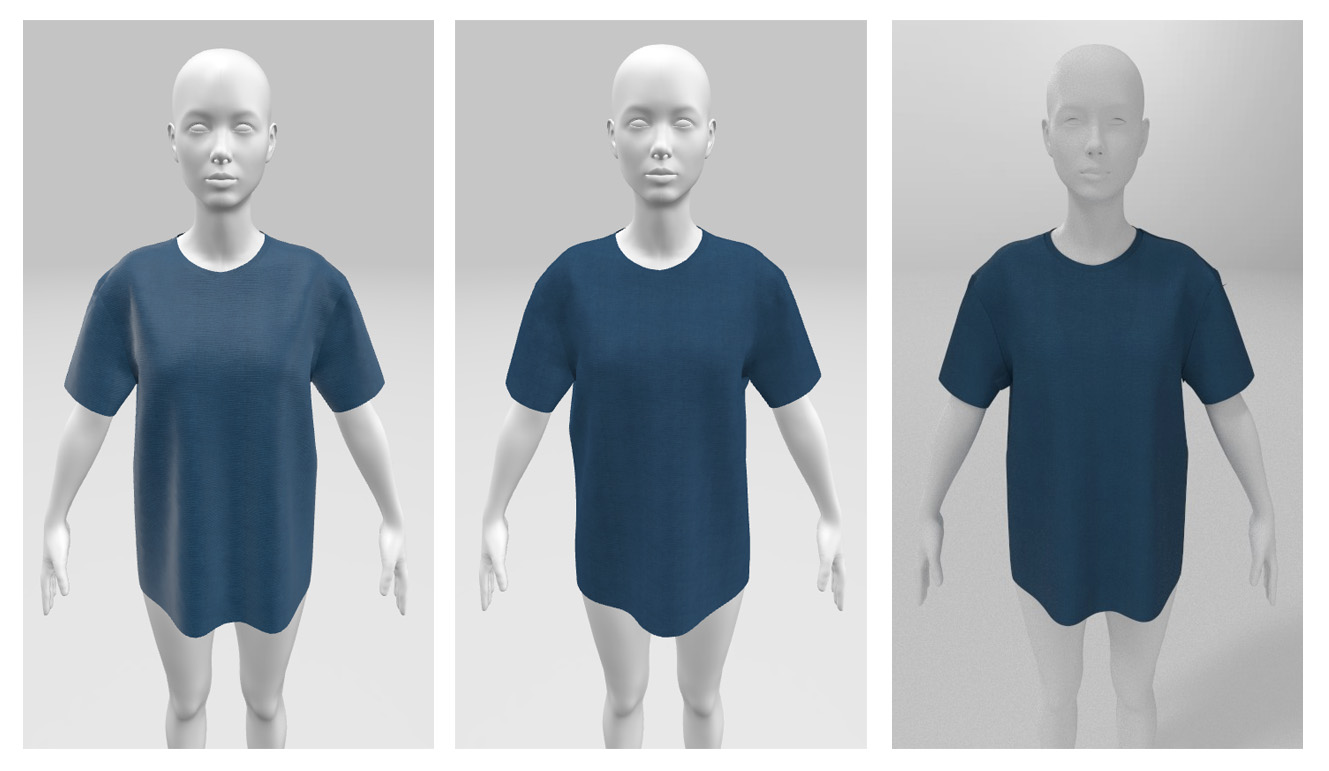
\includegraphics[scale=0.3]{results/lenda}}
    \caption{Tejido de canvas renderizado con \textit{MeshPhysicalMaterial}, \textit{MeshClothMaterial} y el servicio de renderizado de trazado de rayos de Seddi}
\end{figure}

Mientras que el brillo especular de \textit{MeshPhysicalMaterial} da al tejido un aspecto de pl\'astico, el mayor control sobre
el especular de \textit{MeshClothMaterial} permite atenuar el efecto consiguiendo una mayor coherencia con los resultados obtenidos
por el servicio de renderizado en la nube de Seddi.

\begin{figure}[H]
  \vspace{0.5cm}
  \centering
    \frame{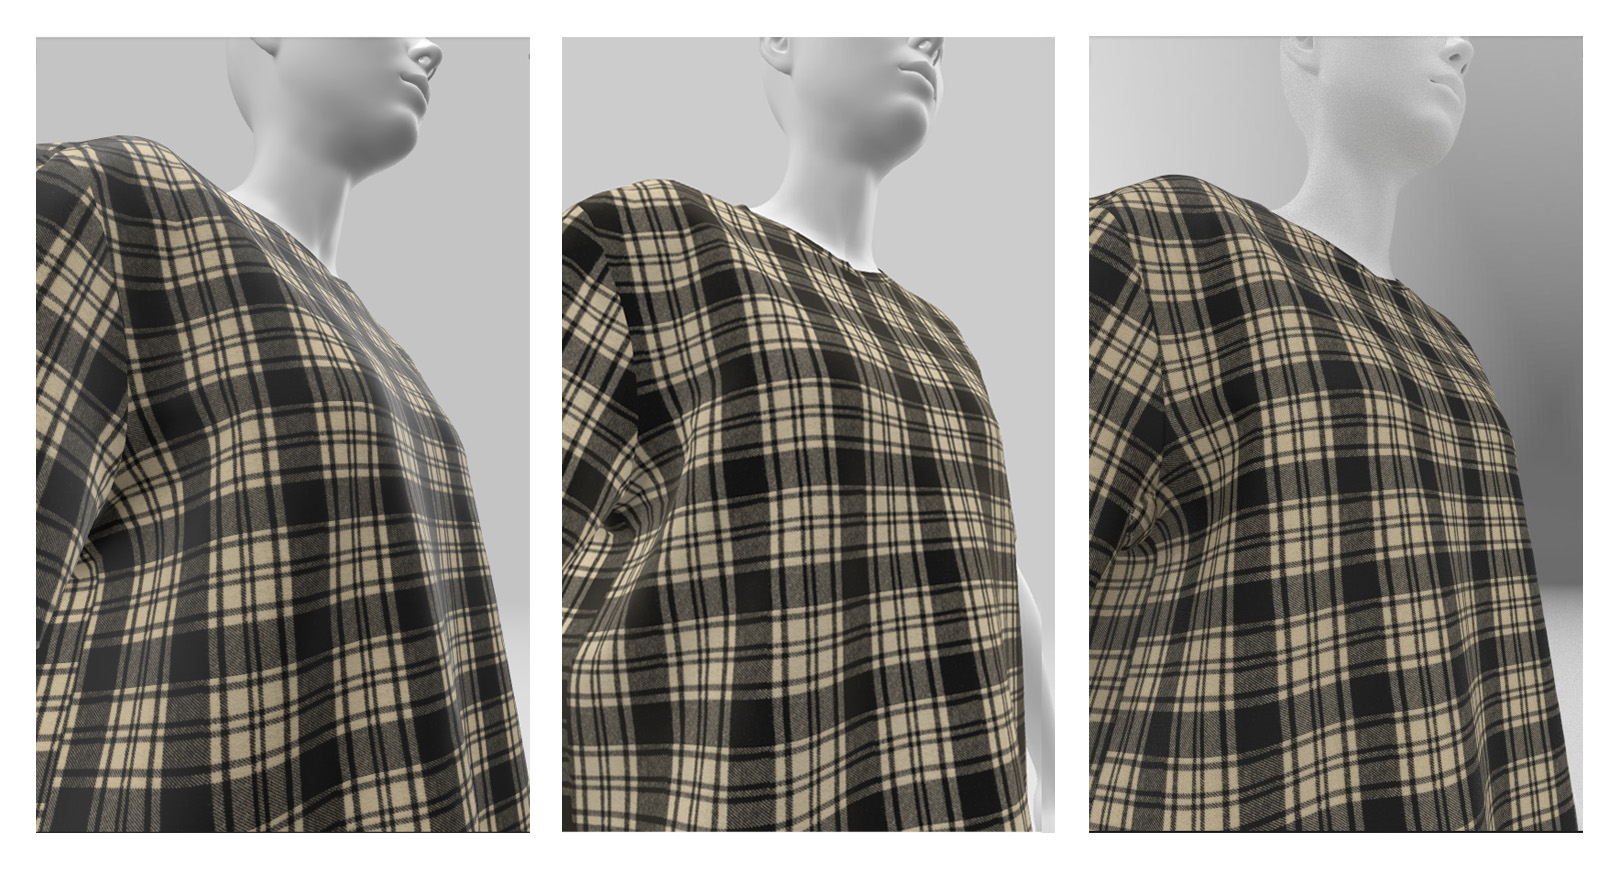
\includegraphics[scale=0.2458]{results/tartantwillbrushed}}
    \caption{Tejido de sarga renderizado con \textit{MeshPhysicalMaterial}, \textit{MeshClothMaterial} y el servicio de renderizado de trazado de rayos de Seddi}
\end{figure}

De igual forma, en la figura 5.11, se aprecia como el \textit{MeshPhysicalMaterial} falla al capturar un tejido de sarga, cuyas reflexiones
son muy definidas el \'angulo cr\'itico. Por su parte, el \textit{MeshPhysicalMaterial} utiliza un color marr\'on con
muy baja luminosidad que aten\'ua el efecto consiguiendo un resultado m\'as parecido al obtenido por el motor de trazado de rayos.
